\section{Rosemary-based Design}
\label{reuse-rosemary}


Compared to the functional design (section \ref{function-design}) the most critical part of the system, data management, is mostly covered by Rosemary.
Datasets are bound to \emph{workspaces}, which have an owner and members that can all view the data inside, effectively restricting data access.
To enable  search and filtering, a specific model for raw data storage is used and supplemented with an extensive tagging system.
The flexibility of this system means that part of the request and the whole data management requirements can be implemented with minimal changes.

User management can be totally reused, but it will need extensions to provide for the necessary user roles.
Furthermore, request and publication management will need to be introduced into the system.

\begin{figure}[!hb]
	\centering
	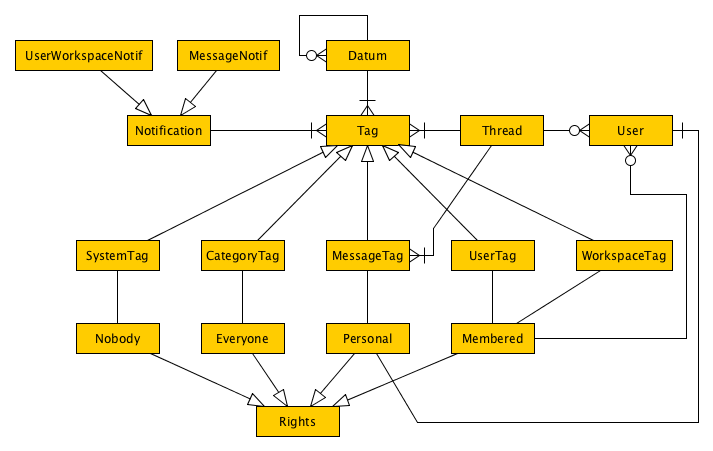
\includegraphics[width=1.0\linewidth]{images/datamodel-clean}
	\caption{
		Rosemary data model with domain specific items removed.
		Describes the workspace, tagging, datum, and notification models.
		The unedited Rosemary data model can be found in appendix \ref{unedited-datamodel}.
	}
	\label{fig:reuse-rosemary-dm}
\end{figure}

\silvia{i believe that from here you actually describe the prototype. keep clear what was rosemary, what is new, or what has been adapted. maybe it is not so relvant to stress the differences, but to have a complete and understandable explantion of what you have done}
\paragraph{Data model}
Figure \ref{fig:reuse-rosemary-dm} depicts the Rosemary data model where the (\ie{} domain specific) items are removed.
%A full view of the data model can be seen in appendix \ref{unedited-datamodel}.
Implementation is done in mongoDB, a document-oriented database \cite{}.
\silvia{present the main entities of the model here. the figure should stay in the body}
The data model and its implementation provide some interesting possibilities.
%What is described in figure \ref{fig:reuse-rosemary-dm} 
A {\tt Datum} is a single piece of raw data, \ie{} a row in a relational database.
This data can be tracked and reused endlessly by applying a {\tt Tag} object.
For example, access control can be applied by tagging a {\tt Datum} with a {\tt WorkspaceTag} which is owned by a {\tt User}.
Many different constructs of this sort can be achieved without ever touching the structure of the actual model itself.
The reuse in the \ivfsystem{} relies heavily on this concept, which means only slight changed had to be made to the original data objects.